%!TEX ROOT=../ctutest.tex
% UZAVŘENO! ÚPRAVY JEN ŽIVOTNĚ NUTNÉ NEBO VE ZBYLÉM ČASE
\chapter{The AIC/FactCheck Context}
\label{chap:pipeline}
Now that we have collected and validated two training, development and testing datasets in chapers~\ref{chap:collection} and~\ref{chap:dataset}, let us spend a short chapter on how this data is being practically used to build a fact verifier under the appropriate knowledge base.

We will explore the works of~\cite{gazo,dedkova} and~\cite{rypar}, our colleagues from the research group \textsf{FactCheck} at \textsf{AIC}, to establish how the \textit{document retrieval} subproblem is being solved, and outline the format and characteristics of its output. This will be referred to in Chapter~\ref{chap:nli} on Natural Language Inference, which takes a claim and a set of evidence on its input and outputs a veracity verdict from $\{\texttt{SUPPORTS},\texttt{REFUTES},\texttt{NOT ENOUGH INFO}\}$.

We will also briefly discuss the \"{end user} application demonstrations we have prepared for the fact-checking task and its subroutines in the past, to specify how the outputs of the following chapters shall be used in practice.

\section{Document retrieval task}
\label{sec:document-retrieval}
During the summer semester 2021, we have subdivided the \textit{fact-checking pipeline} tasks from Figure~\ref{fig:pipeline} among the members of our team, as described in~\ref{sec:subdivision}. While our work is held accountable for the software engineering, experiment design and the validation schemes neccessary for establishing the Czech fact-checking datasets, the work of~\cite{rypar}\footnote{The works of~\cite{gazo} and~\cite{dedkova} were postponed to a later deadline, partly due to the distance learning during the Czech COVID-19 surge, and did not yet deliver a solution to experiment with.} takes their snapshots and uses them to train and validate the Document Retrieval models.

The Document Retrieval model takes a textual claim on input and outputs a set of Documents (e.g. \textsf{ČTK} paragraphs or \textsf{Wikipedia} abstracts) from a fixed domain -- the \textit{knowledge base}. We refer to its result as to the \textit{evidence set}, as it shadows the concept of evidence sets introduced in Figure~\ref{fig:evidence} and present in our datasets (though in~\ref{sec:recall}, we will argue that we only need a reasonable-sized \textit{superset} of the dataset-like evidence set).

To follow up, we dedicate the current Part of our thesis to train a model which, given such an evidence set on its input along with a textual claim, outputs a veracity label to conclude the fact-checking verdict. Therefore, we find it vital for the text of our thesis, to include a brief look into the previous task on the pipeline and see the models that, in the end-applications will be feeding their output into our Natural Language Inference model (Chapter~\ref{chap:nli}) and examine its form and reliability.



\subsection{Recall Over Precision}
\label{sec:recall}
The standard metrics for the retrieval task are the \textit{Precision} and the \textit{Recall}. Loosely speaking, precision characterizes the overall \textit{quality} of the results as the percentage of relevant results in the entire output ($precision=\frac{true~positives}{true~positives + false~positives}$) whereas the recall expresses the \textit{quantity} of the relevant results, as the percentage of the \textit{retrieved} relevant results in the set of \textit{all} relevant results w.r.t. dataset ($recall=\frac{tp}{tp+false~negatives}$). Their \textit{harmonic mean} is called the $F_1$-score, and is commonly used for measuring the quality of the Retrieval models, as it punishes the unwanted \textit{tradeoffs} between \textit{precision} and \textit{recall}.

For us, this is not the case -- due to the \textit{self-attention} mechanism described in~\ref{sec:transformers}, we presume the NLI models to be rather forgiving to the precision faults, i.e. to be able to find the conclusive part of evidence even in a rather long input. Therefore, we use the \textit{recall} as our default benchmark for the Document Retrieval models trained by~\cite{rypar} and~\cite{michal}, as even the task of scaling down the entire \textsf{ČTK db} from $10^8$ paragraphs to, say, a set of $20$, that are guaranteed to contain an \textit{evidence set} yields an admissible input for the NLI models discussed in Chapter~\ref{chap:nli}.

\subsection{Internal State of the Art}

\begin{table}[H] {\techbf{FEVER CS dev set}}
\begin{ctucolortab}\begin{tabularx}{.95\textwidth}{lrrrrr}
    \toprule
                               model &    R@1 &    R@2 &    R@5 &   R@10 &   R@20  \\
    \midrule
                                \textsf{DRQA} &  38.99 &  51.68 &  63.74 &  69.85 &  74.66  \\
             \textsf{Anserini BM25 finetuned} &  39.30 &  49.94 &  61.13 &  67.78 &  73.07 \\
                       \textbf{\textsf{mBERT BFS+ICT}} &  \textbf{61.48} &  \textbf{75.62} &  \textbf{87.34} &  \textbf{91.88} &  \textbf{94.40}  \\
           \textsf{ColBERT\_128dim (FEVER CS)} &  51.64 &  62.84 &  71.32 &  75.22 &  78.28  \\
     \textsf{ColBERT\_128dim (ČTK + FEVER CS)} &  43.71 &  54.59 &  64.84 &  70.87 &  75.28  \\
      \textsf{ColBERT\_64dim (ČTK + FEVER CS)} &  41.31 &  51.53 &  61.37 &  67.19 &  72.02  \\
    \bottomrule
    \end{tabularx}
\end{ctucolortab}

~

\centering{\techbf{ČTK v2.1 test set}}

    
\begin{ctucolortab}\begin{tabularx}{.95\textwidth}{lrrrrr}
    \toprule
                              model &    R@1 &    R@2 &    R@5 &   R@10 &   R@20  \\
    \midrule
                               \textsf{DRQA} &  12.75 &  19.25 &  25.50 &  31.00 &  35.50  \\
            \textsf{Anserini BM25 finetuned} &  15.75 &  22.00 &  29.25 &  33.75 &  39.75  \\
          \textbf{\textsf{ColBERT (FEVER CS + ČTK)}} &  \textbf{19.50} &  \textbf{27.25} &  \textbf{35.25} &  \textbf{40.00} &  \textbf{46.00} \\
     \textsf{mBERT BFS+ICT (FEVER CS + ČTK)} &   1.00 &   2.25 &   5.00 &   8.25 &  12.25 \\
    \bottomrule
    \end{tabularx}
\end{ctucolortab}

    \caption[Recall for a fixed output size of $k$ paragraphs, measured using the \textsf{FEVER CS} and \textsf{ČTK} datasets]{Percent-recall for a fixed output size of $k$ paragraphs, measured using the \textsf{FEVER CS} and \textsf{ČTK} datasets. Reprinted from~\cite{rypar}, bold values signify the best result.}
    \label{tab:dr}
\end{table} % rypar


In Table~\ref{tab:dr}, we show the measurements of the \textit{recall}\footnote{For the less task-relevant (but more standard) $F_1$ measure, see the work of~\cite{rypar}, linked in the Bibliography.} of most significant retrieval models trained by~\cite{rypar} and \cite{michal} from \textsf{AIC}, using the computing power of the \textsf{RCI Cluster}. Even though the numerical models, such as \textsf{DrQA} (\textit{tf--idf}) and the \textsf{Anserini} implementation of \textsf{Okapi BM25} (\textit{bag-of-words})  methods set a strong baseline to validate the Transformer training, they are ultimately surpassed by the neural \textsf{BERT}-like models.


\textsf{AIC CTU}'s internal sota for Document retrieval is a \textit{two-tower retrieval model}~\cite{twotower} based on \textsf{mBERT}~\cite{devlin2019bert}, pretrained on Czech \textsf{Wikipedia} corpus using the Body First Selection and Inverse Cloze tasks, which achieves a \textbf{91.88\%} test recall on the \textsf{FEVER CS} data for a fixed output size of 10 documents.

For the \textsf{ČTK Paragraph} retrieval, Rýpar proposes a \textsf{ColBERT}~\cite{colbert} model trained using $(claim,evidence~document,non{\text -}evidence~document)$ triples from both the \textsf{FEVER CS} and the \textsf{ČTK} dataset, which has a \textbf{40\%} recall at 10 output documents. The \textsf{ČTK} dataset is to be further examined for faults, as the \textsf{mBERT} recall is shockingly low on it, given it was this very model to compute significant part of the \textit{knowledge scopes} (\ref{sec:knowledge-scopes}).

\section{Production}
\subsection[FEVER CS Baseline]{FEVER CS Baseline (Sep 2020)}

In the \textit{Software or Research Project} precedent to this thesis, we have released a baseline \textsf{FLASK} \textsf{API} that performs the end-to-end fact verification (as shown in \ref{fig:pipeline}) of any given textual claim using the \textsf{CS Wikipedia} knowledge base. It follows the format for the \textsf{FEVER} shared task submissions~\cite{fever1} and it is fully containerized to run using a simple \textsf{docker} or \textsf{singularity} \texttt{run} command. It can be run directly from the \textsf{DockerHub}  \texttt{ullriher/fever-cs-baseline} repository, or built from the source\footnote{\url{https://github.com/aic-factcheck/fever-cs-dataset}}. The published \textit{baseline} system uses dated models -- the \textsf{DrQA} for Document Retrieval and a \textit{Decomposable Attention model} for the Natural Language Inference -- which are to be updated with the solutions proposed by of our current research (Chapter~\ref{chap:conclusion}). We include it for a tangible example of product utilizing our theoretical findings and show an example server interaction in Figure~\ref{fig:rys}.

%--- FIG: UTF forms
\begin{figure}[H]
\vspace{2em}
\makebox[\textwidth][c]{\fcolorbox{ctublue}{white}{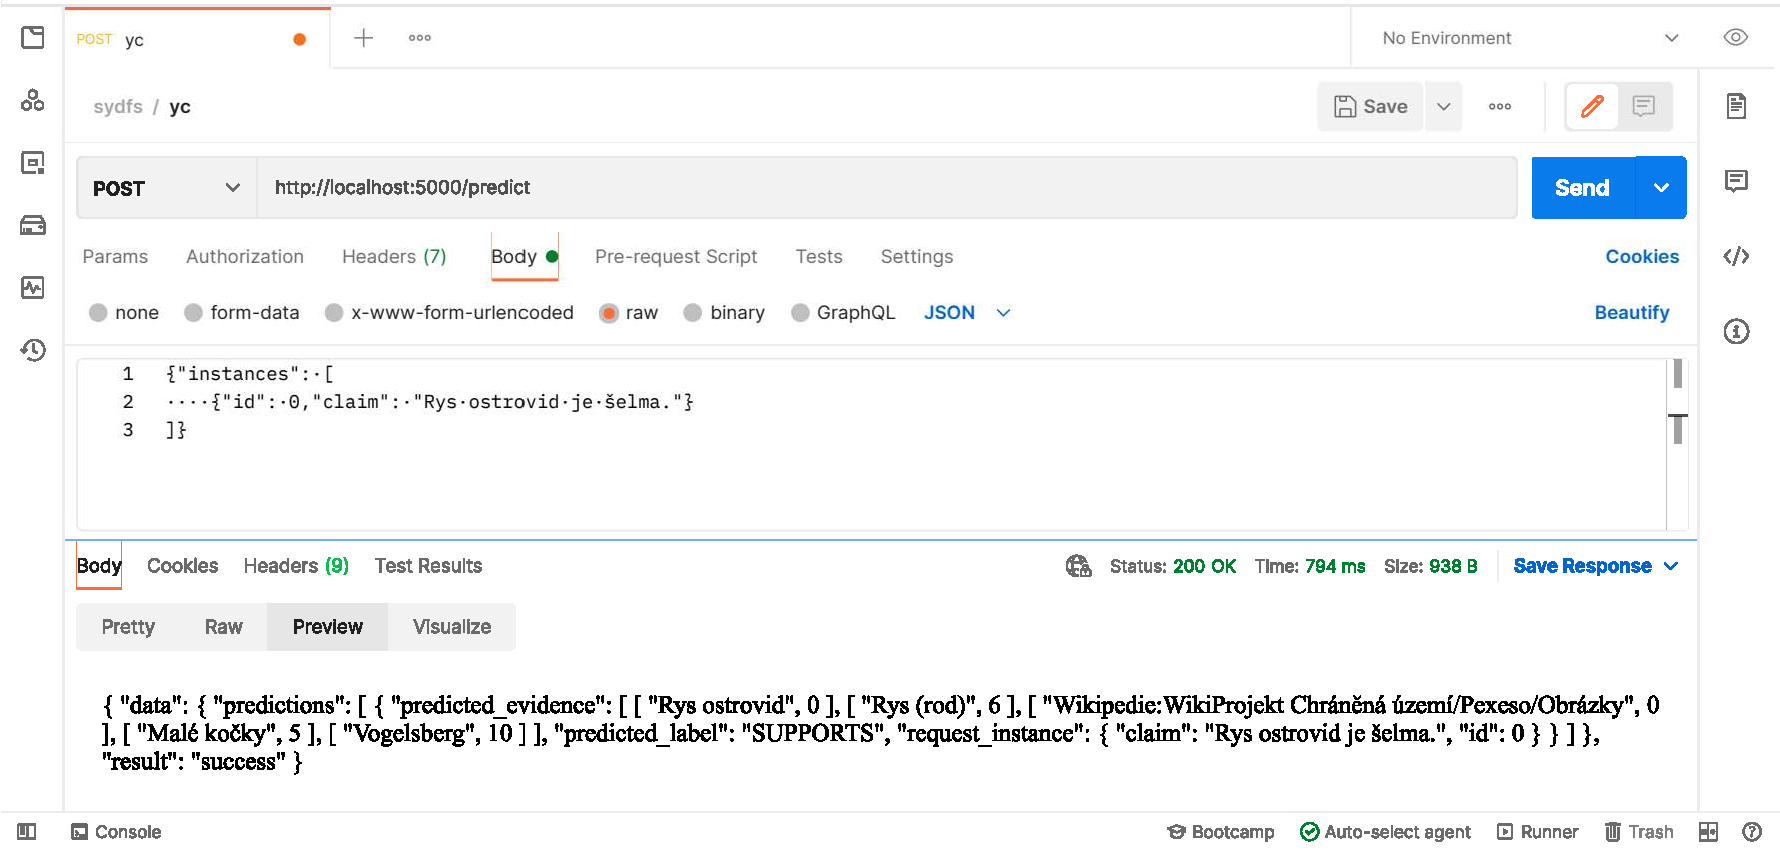
\includegraphics[width=18cm]{fig/rys.pdf}}}
\caption{Our \textsf{fever-cs-baseline} \textsf{API}, accessed through \textsf{Postman}}
\label{fig:rys}
\end{figure}
%--- /FIG

\subsection{Fact Search}


Through the course of the last year, our team supervisor Jan Drchal has produced a plethora of demonstrative production-like interfaces for our meetings with the \textsf{FSS} and \textsf{TAČR} stakeholders. The most notable interface is the \textsf{Fact Search} web console (Figure~\ref{fig:factsearch}) that emulates the outputs of the Document Retrieval task for an arbitrary claim, knowledge base and DR model.  

It computes the single-paragraph inference label using a legacy model for RTE (also known as NLI) for each retrieved document, to show the NLI use case. It also illustrates the Document Retrieval task referred to in~\ref{sec:document-retrieval} and gives a real-world example of an input data for our next chapter\dots

%--- FIG: UTF forms
\begin{figure}[H]
\vspace{2em}
\makebox[\textwidth][c]{\fcolorbox{ctublue}{white}{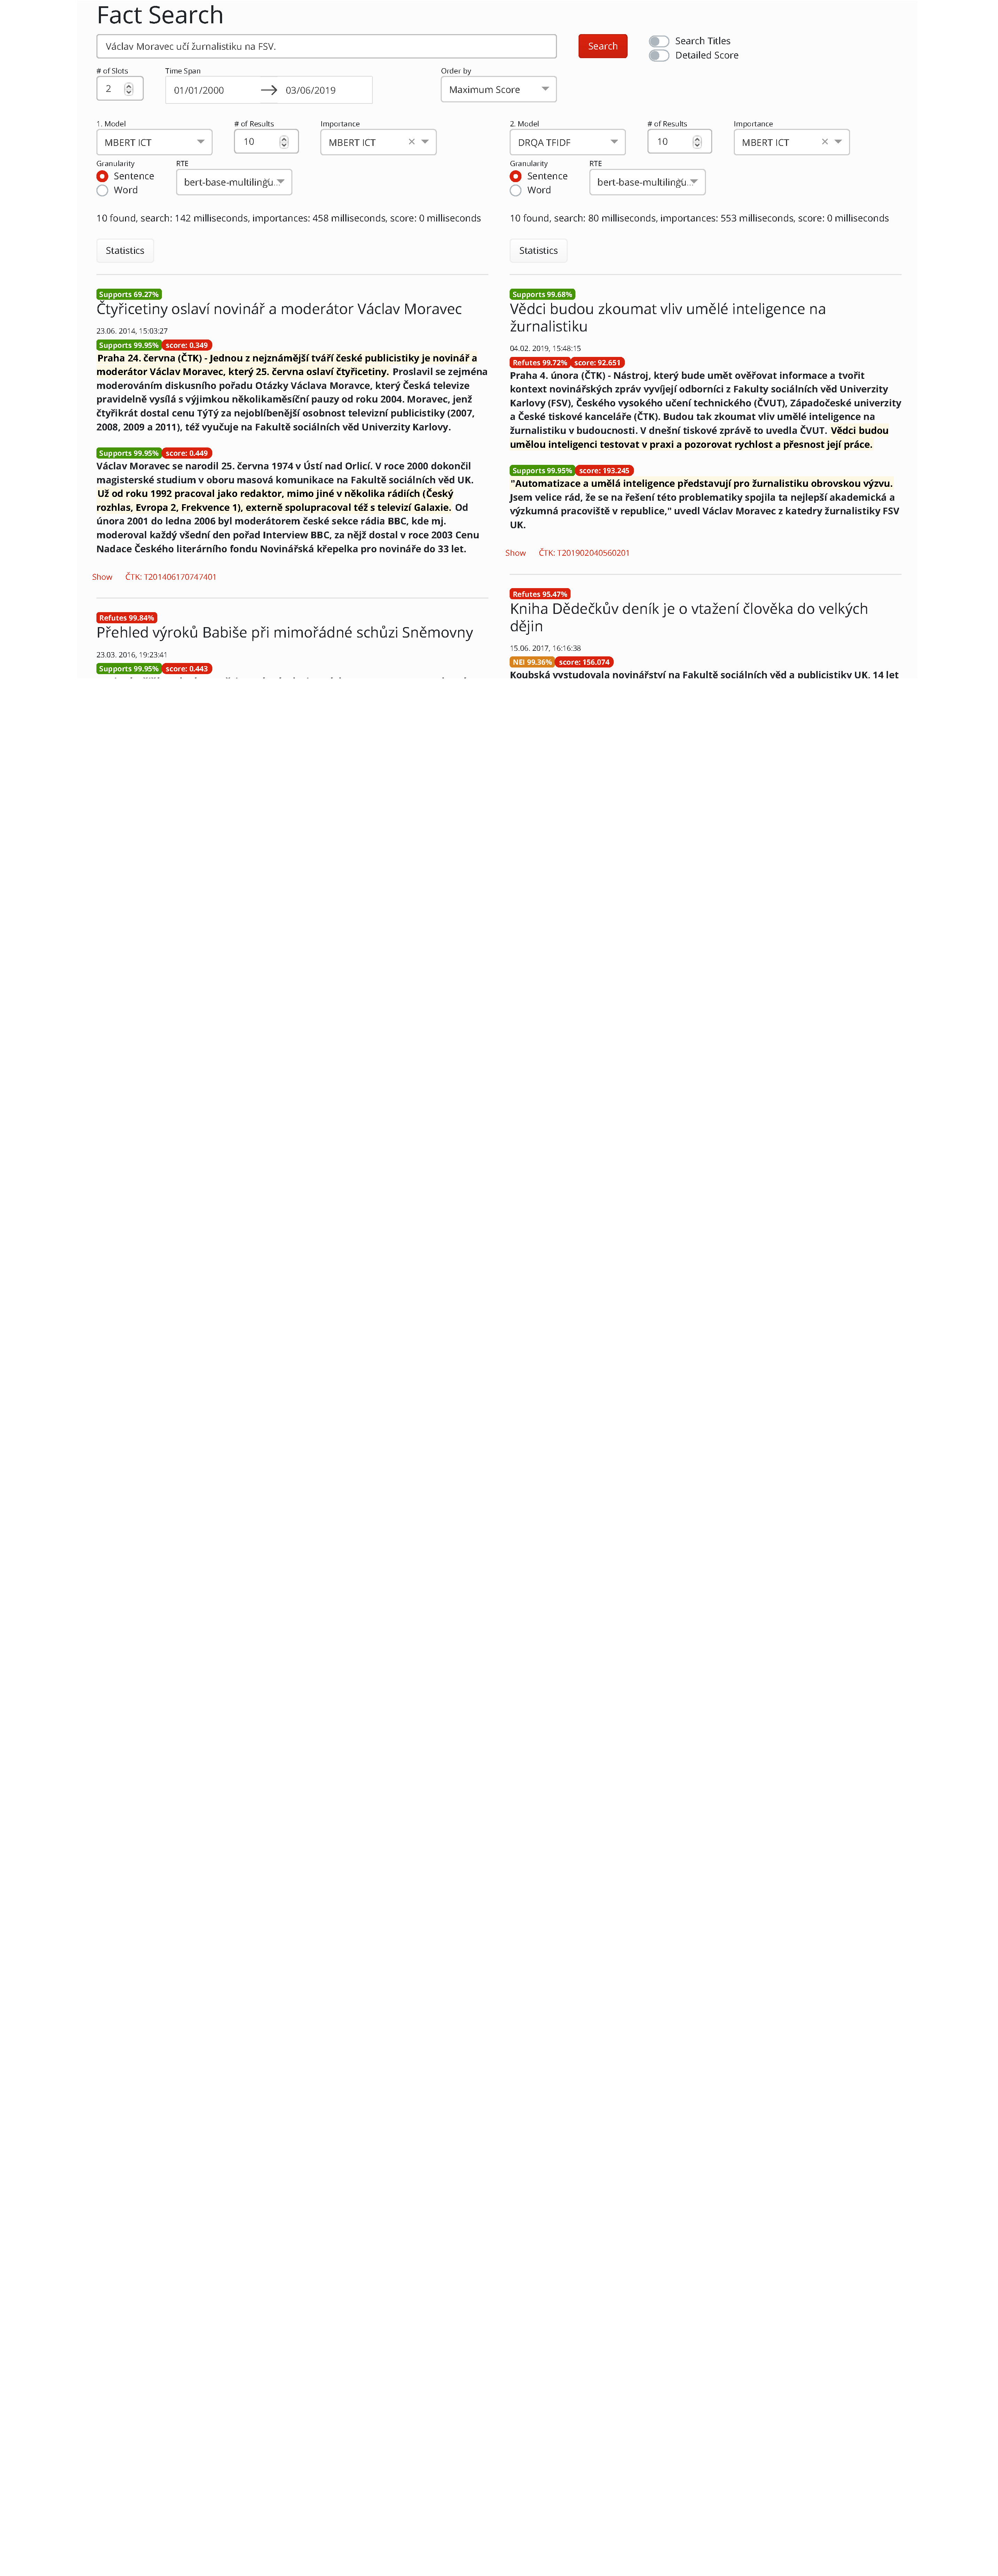
\includegraphics[width=17cm]{fig/factsearch.pdf}}}
\caption{\textsf{Fact Search} demo, authored by Jan Drchal, code at~\cite{honzagit}}
\label{fig:factsearch}
\end{figure}
%--- /FIG
